%!TEX root = ../main.tex
\section{Ableiten von Unterseiten}
Mit dem Festlegen bestimmter Parameter wie Font, Textsatz, Farben, Struktur etc. kann nun damit begonnen werden einige Unterseiten zu erstellen. Durch den Einsatz von Präprozessoren (wie an späterer Stelle im Kapitel \ref{chapter:prepros} auf Seite \ref{chapter:prepros} näher erläutert) gestaltet sich dieser Vorgang sehr modular. Aus diesem Grund wird an dieser Stelle lediglich kurz auf besondere Typen von Inhaltsblöcken eingegangen.

\begin{figure} [h]
	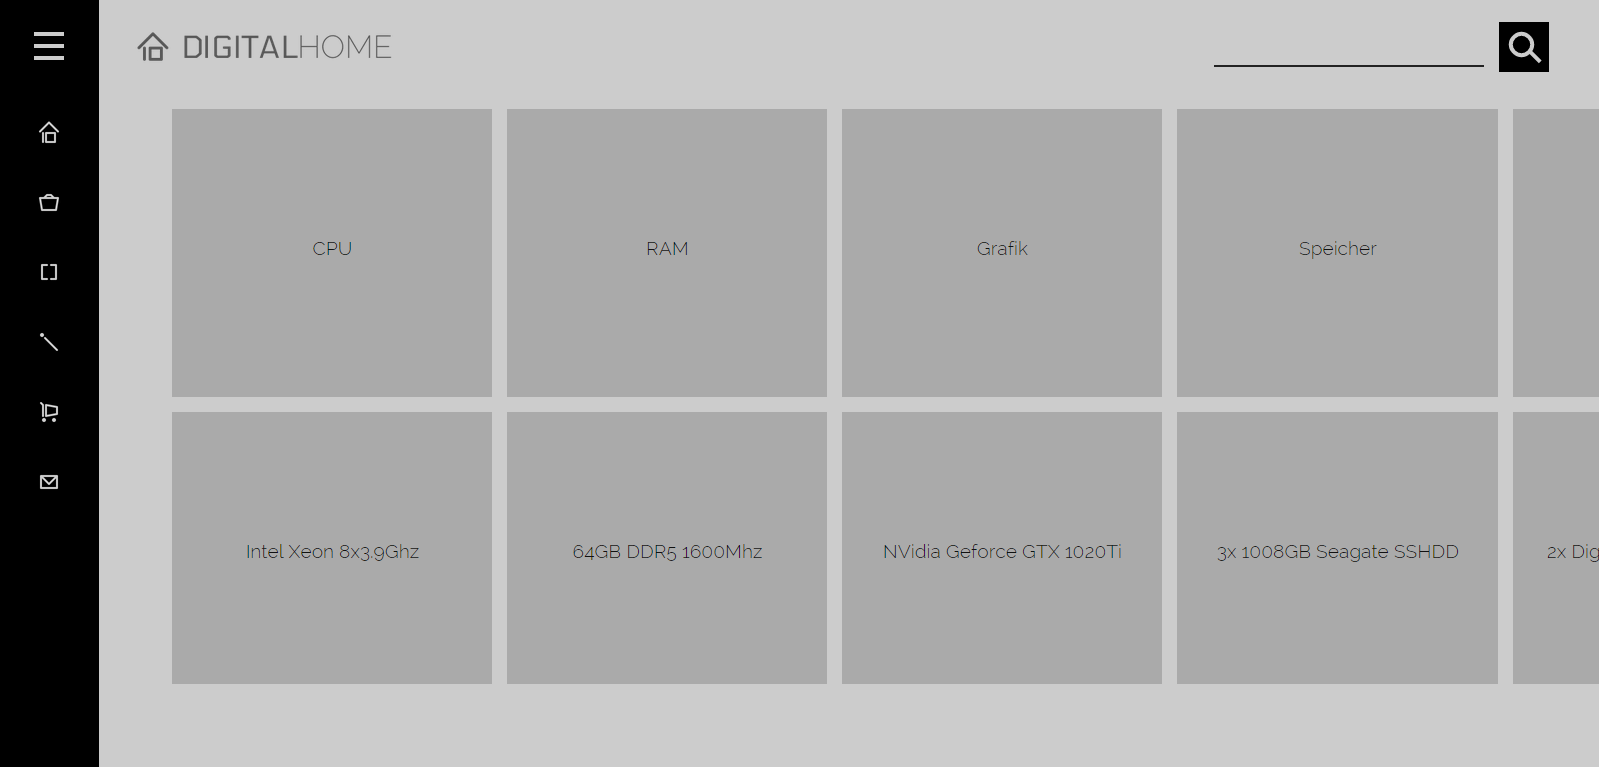
\includegraphics[width=\textwidth]{./img/unters_details.png}
	\caption{Detailbereich mit näheren Informationen zu den Spezifikationen.}
	\label{unters:details}
\end{figure}

Auf der Titelseite befindet sich eine Intro-Bild-Section, die an sich einen halben Inhaltsblock darstellt, indem ein Bild auf voller Größe dargestellt wird. Außerdem liegen hier ansonsten Überschrift- und Textblöcke in denen Informationen für den Benutzer ihren Platz finden.

Die Shop-Seite erhält ebenfalls ein Bild in halber Breite am Anfang der Seite. Danach folgt auch hier wieder ein Überschriften-Block. Anschließend werden die Produkte in einem Kachellayout dargestellt ähnlich den Kacheln in Abbildung \ref{unters:impress}.

\begin{figure} [h]
	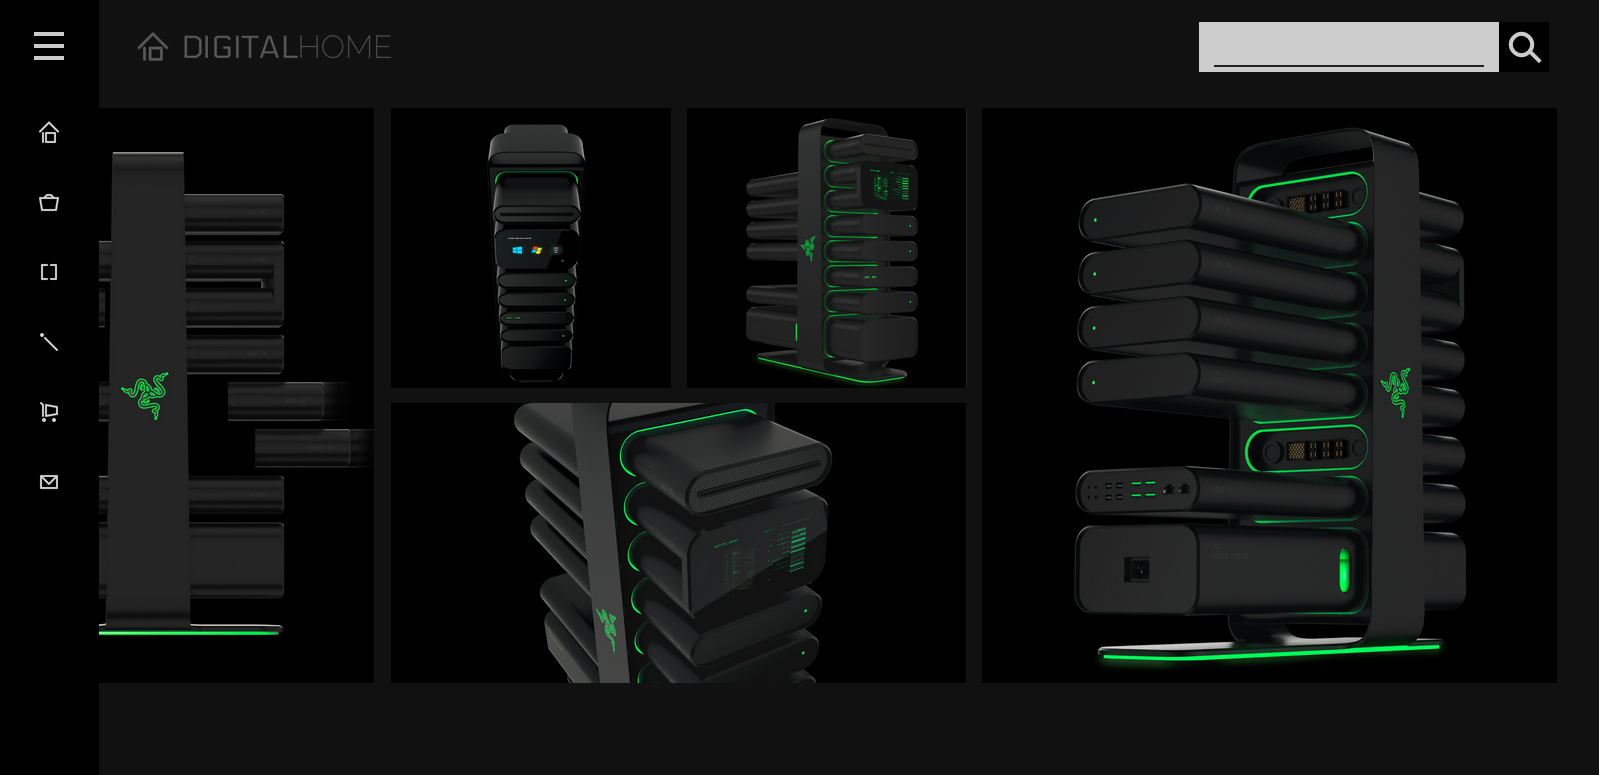
\includegraphics[width=\textwidth]{./img/unters_impress.png}
	\caption{Kachelbereich mit Impressionen zum Produkt.}
	\label{unters:impress}
\end{figure}

Auf den Artikelseiten steht die Information im Vordergrund. Der Nutzer soll schnell zu einem Kauf überzeugt werden. Daher gibt es auf dieser Unterseite einen tabellenartigen Kachelbereich mit genaueren Informationen zum Produkt (Siehe Abbildung \ref{unters:details}). Im Anschluss daran folgt ein dynamischer Kachelbereich mit Impressionen als weiterer Faktor der Überzeugung (Siehe Abbildung \ref{unters:impress}).

Sollte eine Seite bzw. ein Feature nicht implementiert sein, wird der Nutzer auf eine extra für diesen Zweck angelegte Seite weitergeleitet. Auf dieser erhält er die Information über den aktuellen Status der Entwicklung (Zu sehen in Abbildung \ref{unters:err}).

\begin{figure} [h]
	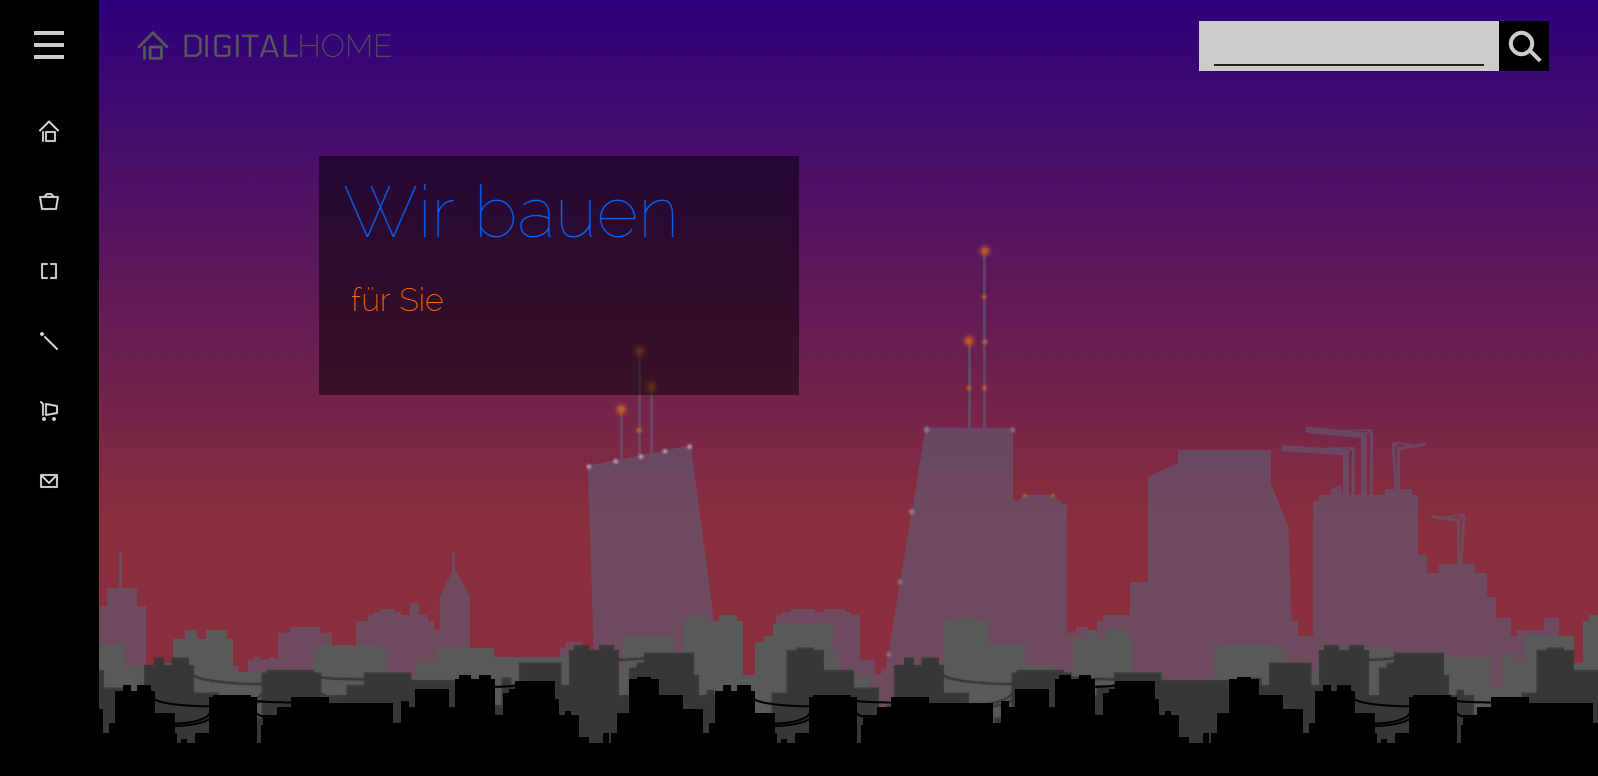
\includegraphics[width=\textwidth]{./img/unters_err.png}
	\caption{Errorseite mit kleinem Hinweis für den Nutzer.}
	\label{unters:err}
\end{figure}